\section{Μέρος Α': Πειραματική Αξιολόγηση}
\subsection{Ερώτημα 3-1-1}

Στο τμήμα αυτό της άσκησης εκτελέστηκαν οι προσομοιώσεις του προγράμματος για όλους τους
ακόλουθους συνδυασμούς:
\begin{itemize}
   \item 
      εκδόσεις προγράμματος: 
      \begin{itemize}
         \item TAS\_CAS
         \item TAS\_TS
         \item TTAS\_CAS
         \item TTAS\_TS
         \item MUTEX
      \end{itemize}
   \item
      iterations: 1000
   \item 
      nthreads: 1, 2, 4, 8, 16 (σε σύστημα με ισάριθμους πυρήνες)
   \item
      grain\_size: 1, 10, 100
\end{itemize}
Ακολουθούν τα σχετικά διαγράμματα που προέκυψαν με βάση τα αρχεία sim.out για τις διαφορετικε παραμέτρους προσομοίωσης:


\begin{minipage}{\textwidth}
   \begin{center}
      \fbox{\textlatin{\textbf{\textit{Grain Size: 1}}}}\\
      \vspace{3mm}
      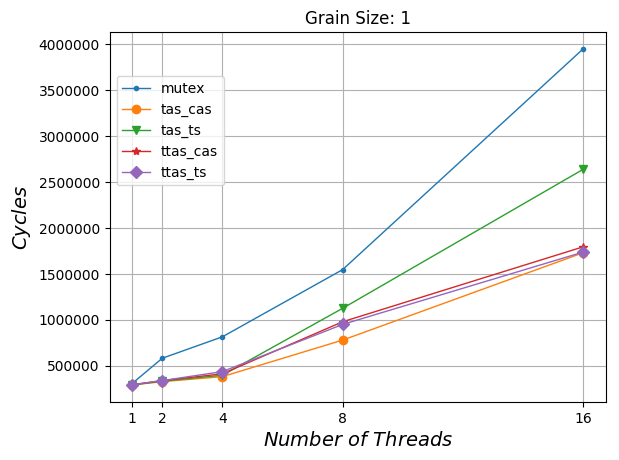
\includegraphics[width=0.7\textwidth, frame]{./graphs/sniper/cycles/grain-1.png}
      \vspace{6mm}
   \end{center}
\end{minipage}

\begin{minipage}{\textwidth}
   \begin{center}
      \fbox{\textlatin{\textbf{\textit{Grain Size: 10}}}}\\
      \vspace{3mm}
      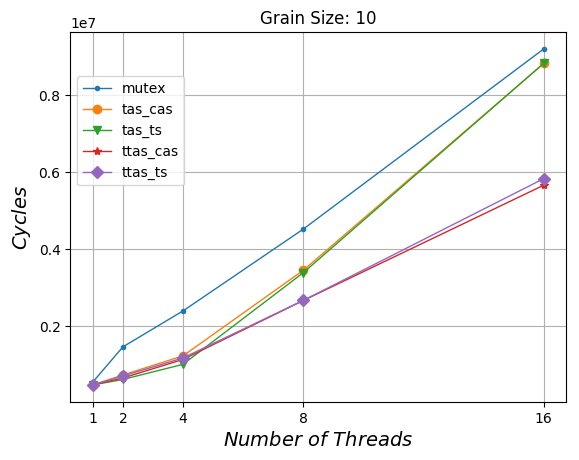
\includegraphics[width=0.7\textwidth, frame]{./graphs/sniper/cycles/grain-10.png}
      \vspace{6mm}
   \end{center}
\end{minipage}

\begin{minipage}{\textwidth}
   \begin{center}
      \fbox{\textlatin{\textbf{\textit{Grain Size: 100}}}}\\
      \vspace{3mm}
      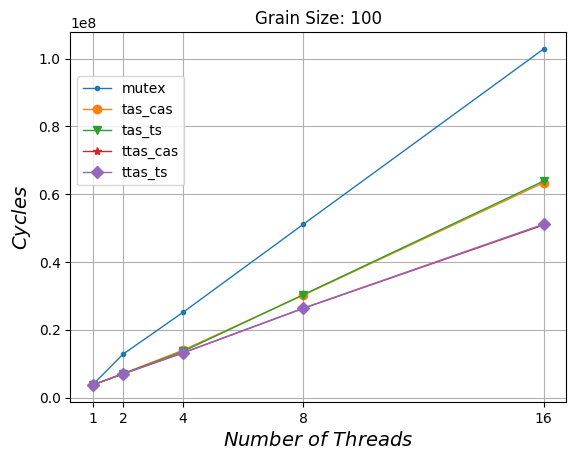
\includegraphics[width=0.7\textwidth, frame]{./graphs/sniper/cycles/grain-100.png}
      \vspace{6mm}
   \end{center}
\end{minipage}

\subsection{Ερώτημα 3-1-2}
\paragraph{Σχόλια - Συμπεράσματα}
Οι μηχανισμοί TAS\_CAS και TAS\_TS υλοποιούν, αμφότεροι το Test-and-set
πρωτόκολλο, απλώς χρησιμοποιούν διαφορετικό τρόπο υλοποίησης. Επομένως
παρουσιάζουν παραπλήσιες επιδόσεις. Όταν 2 ή περισσότεροι επεξεργαστές
προσπαθούν να πάρουν το lock οδηγούνται σε κυκλικές εναλλαγές καταστάσεων
(Modified – Invalid) της cache line που περιέχει το lock, δημιουργώντας αυξημένη
περιττή κίνηση πάνω στο bus. Οι μηχανισμοί TTAS\_CAS και TTAS\_TS υλοποιούν το
πρωτόκολλο Test-and-Test-and-set. Η διαφορά τους με τις Test-and-set υλοποιήσεις
είναι ότι δεν γράφουν συνεχώς πάνω στο lock. Εκτελούν πρώτα ένα load για να δουν
αν είναι ελεύθερο και μόνο τότε δοκιμάζουν το atomic instruction που το γράφει
και προσπαθεί να το δεσμεύσει δηλαδή πρώτα τσεκάρουν το lock και μετά κάνουν
test-and-set. Έτσι σε περίπτωση μη διαθέσιμου lock οι επεξεργαστές κάνουν
spinning τοπικά στην cache τους αποφεύγοντας το άχρηστο broadcasting στον
διάδρομο. Γι αυτό αναμένουμε οι μηχανισμοί Test-and-Test-and-set να πετυχαίνουν καλύτερη
κλιμακωσιμότητα και επίδοση σε σχέση με τους υπόλοιπους.

Μελετώντας τα ανωτέρω διαγράμματα, παρατηρούμε πως ο χρόνος της εκτέλεσης (σε κύκλος) αυξάνεται  σχεδόν γραμμικά με
το πλήθος των νημάτων. Οι ευθείες ωστόσο έχουν διαφορετική κλίση για κάθε
διαφορετικό μηχανισμό συγχρονισμού. Για grain size 1 και 100 την μεγαλύτερη
κλίση (άρα και τη χειρότερη κλιμακωσιμότητα) εχει ο μηχανισμός MUTEX, που
σημαίνει ότι αυξάνει πολύ πιο γρήγορα ο χρόνος εκτέλεσης σε σχέση με τους άλλους
μηχανισμούς. Σε όλα τα grain sizes ωστόσο για το εύρος thread 1 έως 16,
παρατηρούμε πως οι μηχανισμοί σε σειρά βελτιούμενης κλιμακωσιμότητας και
επίδοσης από άποψη χρόνου εκτέλεσης  οι TAS\_TS \& TAS\_CAS και τέλος τα TTAS\_TS
\& TTAS\_CAS. Από όλα τα διαγράμματα γίνεται αντιληπτό ότι την βέλτιστη
κλιμακωσιμότητα -όπως αναμέναμε- σε όλες τις περιπτώσεις επιτυγχάνει ο μηχανισμός
Test-and-Test-and-SET (TTAS) υλοποιημένος είτε με τις ατομικές εντολές
test-and-set ή compare-and-swap.

Σχετικά με το grain size παρατηρείται ότι για grain size 10, οι μηχανισμοί TAS
γιa 16 threads πλησιάζουν στην επίδοση τον μηχανισμό MUTEX. Παρατηρούμε επίσης
πως καθώς αυξάνεται το grain size, δηλαδή το πλήθος των dummy υπολογισμών, τόσο
περισσότερο βελτιώνεται και γίνεται γραμμική με χαμηλότερη κλίση η
κλιμακωσιμότητα των μηχανισμών, και ιδίως για το MUTEX. Αυτό μπορεί να
αιτιολογηθεί, καθώς σπαταλάται πλέον περισσότερος χρόνος για τους υπολογισμούς
και λιγότερος χρόνος για τον ανταγωνισμό του lock, οπότε έχουμε καλύτερη
επίδοση. Σαφώς βέβαια, αφού αυξάνει το πλήθος των dummy υπολογισμών οι χρόνοι
στα αντίστοιχα διαγράμματα μεγαλώνουν κατά μία τάξη μεγέθους (x10) για κάθε
δεκαπλασιασμό του grain size.